%% Paper Overleaf: https://www.overleaf.com/project/6ad46327aacec45bf553b9c0
%% Slides editable source: https://github.com/GreenComp-ERC/ImpactOfFossilFeulPrice/tree/main/conference/ACAIT2026/slides
%% Poster editable source: https://github.com/GreenComp-ERC/ImpactOfFossilFeulPrice/tree/main/conference/ACAIT2026/poster
%% Slides Overleaf-ready ZIP: https://github.com/GreenComp-ERC/ImpactOfFossilFeulPrice/raw/refs/heads/main/conference/ACAIT2026/source_archives/ACAIT2026_Slides_Source.zip
%% Poster Overleaf-ready ZIP: https://github.com/GreenComp-ERC/ImpactOfFossilFeulPrice/raw/refs/heads/main/conference/ACAIT2026/source_archives/ACAIT2026_Poster_Source.zip
%% Overleaf import instructions: see SOURCES.md.
%% Build: latexmk -pdf -interaction=nonstopmode -halt-on-error main.tex
\documentclass[conference]{IEEEtran}

\IEEEoverridecommandlockouts

\usepackage{amsmath}
\usepackage{amssymb}
\usepackage{booktabs}
\usepackage{capt-of}
\usepackage{cite}
\usepackage[T1]{fontenc}
\usepackage{graphicx}
\usepackage{multirow}
\usepackage{flushend}
\usepackage{array}
\usepackage{url}
\usepackage[hidelinks]{hyperref}
\usepackage{tikz}
\usetikzlibrary{arrows.meta,positioning,calc}
\setlength{\tabcolsep}{3.5pt}
\newcolumntype{P}[1]{>{\raggedright\arraybackslash}p{#1}}
\hypersetup{pdftitle={Fossil Fuel Prices and Capital Cost: A Machine Learning Driven Study on Energy Transition},pdfauthor={Shilin Ou, Luyao Zhang, Ming-Chun Huang}}

\graphicspath{{figures/}}
% Native labels over original artwork. Images and numerical curves are unchanged.
\definecolor{PaperModelBlue}{HTML}{173C5B}
\definecolor{PaperXGB}{HTML}{800080}
\newcommand{\PaperNetwork}[2]{%
\resizebox{#1}{!}{\begin{tikzpicture}
\node[anchor=south west,inner sep=0] at (0,0) {\includegraphics[height=5.10cm]{#2}};
\node[fill=PaperModelBlue,text=white,minimum width=0.78cm,minimum height=0.20cm,inner sep=0pt,font=\fontsize{6.2}{7}\selectfont] at (2.11,4.42) {GPR};
\end{tikzpicture}}}
\newcommand{\PaperOilComparison}[2]{%
\resizebox{#1}{!}{\begin{tikzpicture}
\node[anchor=south west,inner sep=0] at (0,0) {\includegraphics[width=12.5cm]{#2}};
\fill[white] (10.97,4.06) rectangle (12.25,5.27);
\draw[black!15,line width=0.4pt] (10.97,4.06) rectangle (12.25,5.27);
\draw[blue,line width=0.7pt] (11.05,5.12)--(11.24,5.12);
\fill[blue] (11.145,5.12) circle (0.018);
\draw[green!45!black,line width=0.9pt] (11.05,4.90)--(11.24,4.90);
\draw[red,dash dot,line width=0.7pt] (11.05,4.68)--(11.24,4.68);
\draw[PaperXGB,densely dotted,line width=0.8pt] (11.05,4.46)--(11.24,4.46);
\draw[orange,line width=0.7pt] (11.05,4.24)--(11.24,4.24);
\foreach \y/\lab in {5.12/Actual,4.90/LSTM-GPR,4.68/SARIMA,4.46/XGBoost,4.24/LightGBM}{
\node[anchor=west,inner sep=0,font=\fontsize{4.7}{5.2}\selectfont] at (11.31,\y) {\lab};}
\end{tikzpicture}}}
\newcommand{\PaperMethodology}[2]{%
\resizebox{#1}{!}{\begin{tikzpicture}[x=1bp,y=1bp]
\node[anchor=south west,inner sep=0] at (0,0) {\includegraphics[width=1313.03992bp]{#2}};
% Correct the summation dummy variable to match the manuscript loss function.
\fill[white] (207,176) rectangle (402,273);
\node[align=center,inner sep=0,font=\fontsize{15}{20}\selectfont] at (304,227) {$\widehat\Theta_h=\arg\min_{\Theta_h}\mathcal L_h$\\[3bp]$\displaystyle\mathcal L_h=\frac{1}{T-h}\sum_{t=1}^{T-h}\varepsilon_t^2$\\[3bp]$\varepsilon_t=y_{t+h}-G(x_t;\Theta_h)$};
\end{tikzpicture}}}


\title{Fossil Fuel Prices and Capital Cost: A Machine Learning Driven Study on Energy Transition}


\author{
\IEEEauthorblockN{Shilin Ou\IEEEauthorrefmark{2},
Luyao Zhang\IEEEauthorrefmark{1},
and Ming-Chun Huang\IEEEauthorrefmark{1}}
\IEEEauthorblockA{Duke Kunshan University\\
Suzhou, China}
\thanks{\IEEEauthorrefmark{1}Corresponding authors: Zhang: luyao.zhang@dukekunshan.edu.cn, Social Science Division and Digital Innovation Research Center; Huang: mingchun.huang@dukekunshan.edu.cn, Natural and Applied Science Division and Digital Innovation Research Center, Duke Kunshan University. Address: No.8 Duke Ave., Kunshan, Jiangsu 215316, China.}
\thanks{\textbf{Acknowledgments}: The Duke Kunshan University Education Development Foundation supports the research. The research results of this article are also sponsored by the Kunshan Municipal Government research funding. \IEEEauthorrefmark{2} Shilin benefited from scholarly exchange with participants in the AAAI-26 Workshop on AI for Environmental Science, held on January 27, 2026, at the Singapore EXPO in Singapore. Shilin gratefully acknowledges the Travel Grant provided by the Duke Kunshan University Office of Academic Services, which supported participation in the workshop.
 }
}





\IEEEaftertitletext{%
\vspace{-1.0em}
\begin{center}
\begin{minipage}{0.96\textwidth}
\centering
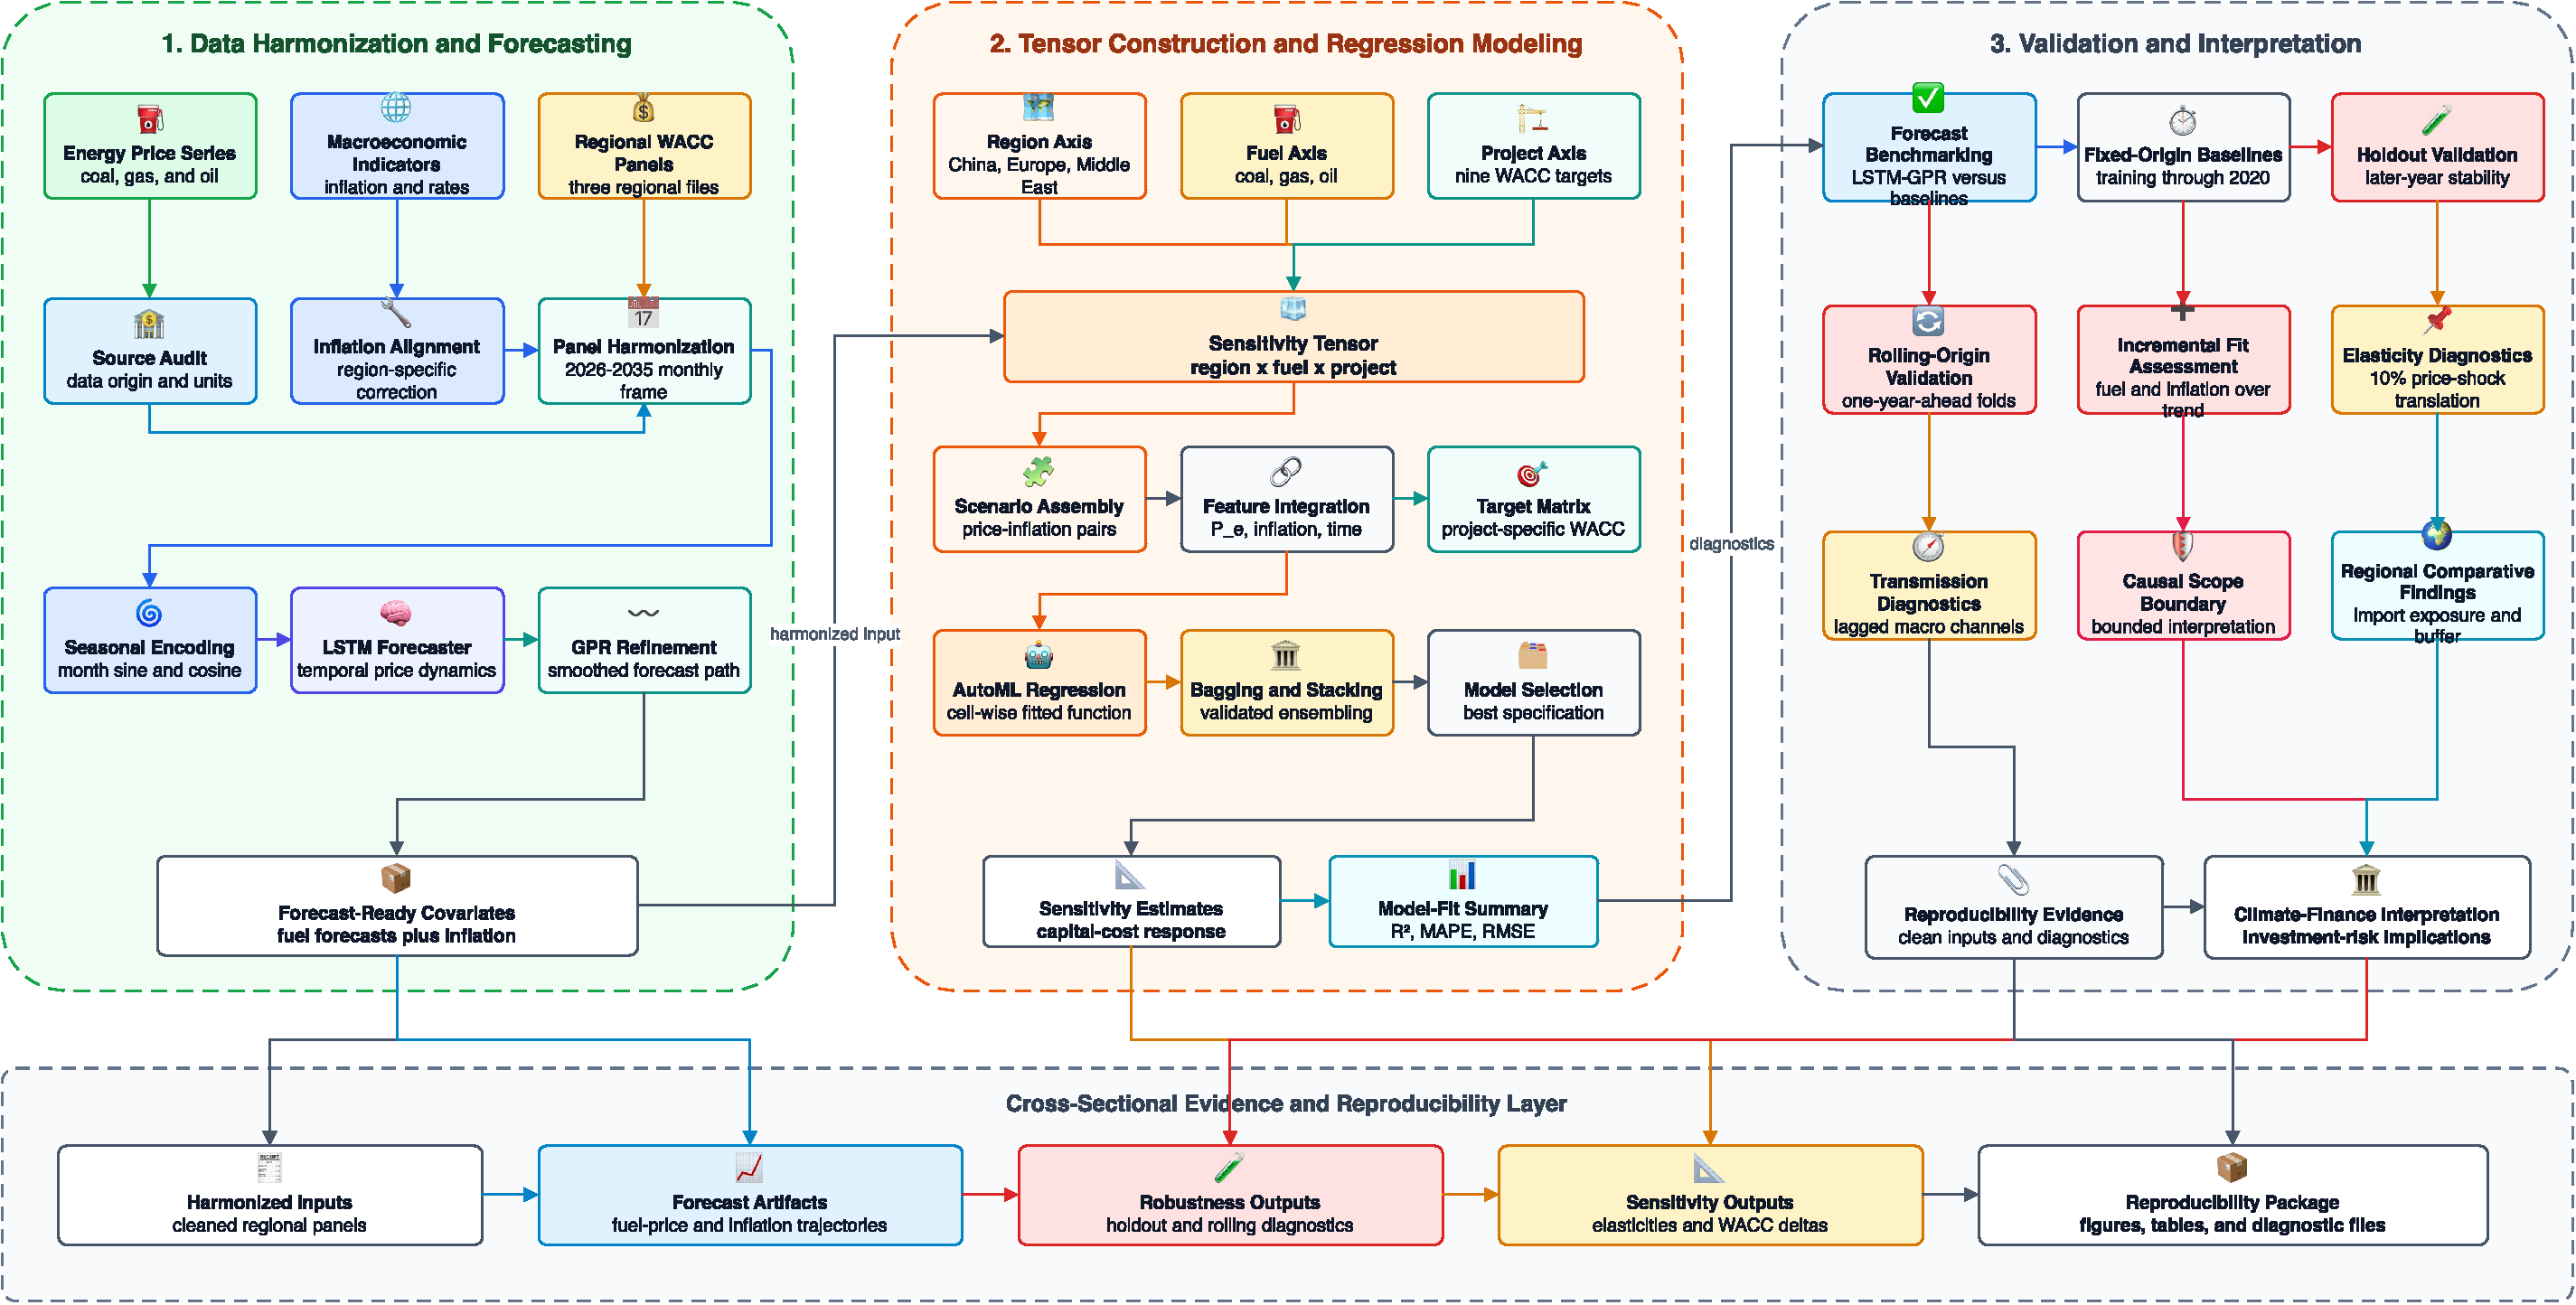
\includegraphics[width=\linewidth]{fossilfuel_wacc_tensor_framework_print.pdf}
\captionof{figure}{End-to-end tensor framework for weighted average cost of capital (WACC) sensitivity analysis. Cleaned fuel, macroeconomic, and regional WACC panels feed a region x fuel x project tensor, regression layer, validation diagnostics, and reproducibility outputs.}
\label{fig:tensor-framework}
\end{minipage}
\end{center}
\vspace{-0.6em}
}

\begin{document}

\maketitle

\begin{abstract}
Financial risk assessment plays a vital role in accelerating the global energy transition and achieving the 1.5$^\circ$C climate target. This study develops a three-stage machine learning framework to analyze the impact of fossil fuel price volatility on the weighted average cost of capital (WACC) for energy transition projects. First, a hybrid Long Short-Term Memory-Gaussian Process Regression (LSTM-GPR) model forecasts fossil fuel prices, followed by an LSTM-based inflation predictor. In the final stage, an AutoML (AutoGluon) regression model evaluates how variations in fossil fuel prices and inflation influence WACC across nine energy sectors and multiple global regions.

The results show regional differences in model fit: average $R^2$ is 0.670 for Europe, 0.650 for China, and 0.547 for the Middle East, with stronger fit for solar and wind projects. These fit statistics describe the joint fuel-price and inflation specifications and do not measure the magnitude of price-shock responses. Additional holdout, rolling-origin, and transmission-diagnostic checks are used to interpret these findings as scenario comparisons and mechanism evidence rather than as formal causal identification. The approach integrates AI-driven forecasting with climate finance modeling, providing an interpretable and data-driven tool to support policy design, green investment strategies, and climate-resilient energy planning.
\end{abstract}

\begin{IEEEkeywords}
Weighted average cost of capital, fossil fuel price volatility, climate finance, energy transition, LSTM-GPR, AutoGluon.
\end{IEEEkeywords}

\section{Introduction}

The urgency of mitigating global warming necessitates a rapid energy transition to achieve the Sustainable Development Goals (SDGs) \cite{messerli2019global}. Energy-system transformation is central to climate-change mitigation \cite{BOGDANOV2021120467}. This transition is not solely a technological endeavor \cite{CHEN20191564}; it also encompasses critical economic dimensions, among which the weighted average cost of capital (WACC) is a critical metric \cite{BACHNER2019100373}. It represents the average return required by capital providers, balancing the costs of debt and equity financing \cite{BACHNER2019100373}. The environmental consequences of this financial indicator are profound; Ameli et al. report 35\% lower green electricity production in Africa under region-specific WACC assumptions in a cost-optimal 2$^\circ$C pathway; their financing-policy scenario allows Africa to reach net-zero emissions approximately ten years earlier \cite{ameli2021higher}.

This study aligns with the UN Sustainable Development Goals (SDGs), specifically SDG 7 (Affordable and Clean Energy) through research on renewable project finance, SDG 13 (Climate Action) by examining financing conditions relevant to decarbonization, SDG 9 (Industry, Innovation and Infrastructure) through an open, reproducible three-stage machine learning pipeline, and SDG 17 (Partnerships for the Goals) by releasing harmonized multi-regional panels to support global research collaboration.

A pernicious challenge for the energy transition is its inherent vulnerability to shocks from the legacy fossil fuel system it seeks to replace. Global oil, gas, and coal price fluctuations can affect inflation and financing conditions, creating potential exposure for capital-intensive renewable projects \cite{melodia2022energy}. Financing assumptions can change modeled investment choices and transition pathways \cite{egli2019bias}. Existing research has examined the relationship between WACC, interest rates, and unstable market conditions in the energy sector \cite{dobrowolski2022weighted}. However, less attention has been devoted to evaluating its influence on WACC within the context of energy transition projects. Additionally, the varied impacts of fossil fuel price volatility across different energy sectors and regions have not been fully explored.

Therefore, this study focuses on the upcoming decade and seeks to answer the following questions:
\begin{itemize}
    \item How do fossil fuel price fluctuations relate to the WACC of energy transition projects in modeled future scenarios?
    \item How do these price dynamics relate to capital costs across regions, particularly between fuel-importing and fuel-exporting countries, and how should financing strategies for low-carbon projects be shaped?
\end{itemize}

This work contributes an open and reproducible AI framework that translates fossil fuel price signals into actionable climate finance intelligence. By organizing regional, fuel, and project comparisons within an AutoGluon-based forecasting pipeline, the framework provides decision support for analyzing regional differences in financing conditions, energy costs, and decarbonization pathways. Its outputs can inform efforts to reduce household energy burdens, improve environmental quality, and support more effective climate and energy policy across diverse global regions.



\textbf{Open Science Statement:} Code, data-processing instructions, cleaned WACC scenario panels, archived forecast comparisons, and corrected sensitivity diagnostics for this version are available in the organization repository\footnote{\url{https://github.com/GreenComp-ERC/ImpactOfFossilFeulPrice}}. An archived dataset snapshot is hosted on Hugging Face\footnote{\url{https://huggingface.co/datasets/global-nomad-nexus/ImpactOfFossilFuelPrice-WACC}}; the repository records the version and provenance of the diagnostics used in this paper. Editable paper, slides, and poster sources are provided in the repository's \texttt{conference/ACAIT2026/} directory.

\section{Literature Review}

\subsection{Calculation of WACC}

For the WACC data, this study mainly uses the dataset from Calcaterra et al. \cite{calcaterra2024reducing}, which contains predictions for WACC across different regions. The calculation begins with analyzing past financial data at the enterprise level, calculating the cost of debt and equity, and incorporating the leverage ratio and tax rate to determine each company's WACC as follows \cite{calcaterra2024reducing}:
\begin{equation}
WACC_{it}=L_{it}\times r_{Dit}\times (1-\mathrm{TaxRate}_{it})+(1-L_{it})\times r_{Eit}.
\end{equation}
where $WACC_{it}$ represents the weighted average cost of capital for firm $i$ at time $t$, $L_{it}$ is the leverage ratio, $r_{Dit}$ is the cost of debt, $r_{Eit}$ is the cost of equity, and $\mathrm{TaxRate}_{it}$ is the tax rate for firm $i$ at time $t$.

The national WACC is then derived by weighting and averaging each company's WACC based on its share of the national utilities-market revenue \cite{calcaterra2024reducing}:
\begin{equation}
WACC_{ct}=\sum_i\left(\frac{\mathrm{Revenue}_{it}}{\mathrm{TotalRevenue}_{ct}}\right)\times WACC_{it}.
\end{equation}
where $WACC_{ct}$ represents the weighted average cost of capital for country $c$ at time $t$, $\mathrm{Revenue}_{it}$ is the revenue of firm $i$ at time $t$, and $\mathrm{TotalRevenue}_{ct}$ is the total utilities-market revenue of country $c$ at time $t$.

After that, Calcaterra et al. \cite{calcaterra2024reducing} introduce a time dimension and financial learning, simulating how technological progress and experience accumulation can lower WACC by reducing technological risks and the required safety margin. The financial-learning scenario models capital costs as a function of cumulative deployment:
\begin{equation}
\mathrm{CoC}_{tnT}=\mathrm{CoC}_{0n,T}\times\left(\frac{Y_{tn,T}}{Y_{0n,T}}\right)^{b_T}.
\end{equation}
where $\mathrm{CoC}_{tnT}$ is the cost of capital for country $n$ at time $t$ and technology $T$, $\mathrm{CoC}_{0n,T}$ is the initial cost of capital, $Y_{tn,T}$ is cumulative technology deployment, $Y_{0n,T}$ is initial technology deployment, and $b_T=\log_2(1-0.05)<0$ is the financial-learning exponent. The separate CoC-convergence scenario models convergence towards developed-country financing conditions by 2050.

Utilizing the aforementioned data and assumptions, it can employ a suite of climate-energy-economy models to simulate the WACC across various regions and energy sectors.

\subsection{Impact of Fossil Fuel Prices on WACC Components}

The previous subsection outlines the calculation of $WACC_{it}$ using firm-level data, in which the cost of equity ($r_{Eit}$) and the cost of debt ($r_{Dit}$) are not static. They are profoundly influenced by broader market dynamics, among which fossil fuel prices play a critical role \cite{melodia2022energy}.

The cost of equity ($r_{Eit}$) is estimated using the Capital Asset Pricing Model (CAPM), defining the expected return as:
\begin{equation}
r_{Eit}=r_{f,t}+\beta_i(r_{m,t}-r_{f,t}).
\end{equation}
where $r_{f,t}$ is the risk-free rate at time $t$, $\beta_i$ is the firm's systematic risk, and $(r_{m,t}-r_{f,t})$ is the equity risk premium (ERP).

Fossil fuel prices could influence the components of the CAPM equation. The substitution effect suggests that higher fossil fuel prices can enhance the economic competitiveness of renewable energy projects and influence perceived risk and the required return, $r_{Eit}$ \cite{Lieberman2007RenewableHedge}. Additionally, the impact on systematic risk ($\beta_i$) is ambiguous. Renewable assets can act as a hedge against fossil fuel price volatility due to their zero fuel cost \cite{Lieberman2007RenewableHedge}. Stock-market evidence varies: Vr\^inceanu et al. find no significant effect of oil-price volatility on renewable-stock return volatility in their sample \cite{vrinceanu2020influence}. Renewable and fossil power portfolios can also differ in financial risk and return, as reported for India \cite{su13052573}.

Similarly, the cost of debt ($r_{Dit}$) is also susceptible to fossil fuel price shocks, which can contribute to inflation \cite{melodia2022energy,millischer2024renewables}. Changes in the interest-rate environment affect economy-wide borrowing costs and WACC \cite{dobrowolski2022weighted}. At the project level, Power Purchase Agreements (PPAs), counterparty risk, and risk-transfer instruments can affect financing conditions and the credit spread component of $r_{Dit}$ \cite{duma2023risk}. Evidence on environmental financial premia is conditional: Wilberg et al. find no aggregate ESG-score effect but an association between the environmental component and lower capital costs \cite{kjellevoll2023impact}.

Therefore, the final calculated $WACC_{it}$ for a renewable energy firm is a function not only of its internal financial structure ($L_{it}$) but also of these external pressures that alter the fundamental costs of its capital ($r_{Eit}$ and $r_{Dit}$). The interplay of these mechanisms is summarized in Table~\ref{tab:channels}. Ultimately, the net impact on the WACC of renewable energy projects hinges on the relative magnitude of these opposing forces: the project-level advantages stemming from higher fossil fuel prices versus the detrimental consequences of macroeconomic contagion.

\begin{table}[t]
\centering
\caption{Theoretical Channels of Fossil Fuel Price Transmission to Renewable Energy WACC}
\label{tab:channels}
\scriptsize
\begin{tabular}{P{0.27\linewidth}P{0.27\linewidth}P{0.34\linewidth}}
\toprule
\textbf{Price Signal} & \textbf{Affected Component} & \textbf{Transmission Channel} \\
\midrule
Level increase & $r_E$ (cost of equity) & Substitution effect \\
Level/volatility & $r_E$ (cost of equity) & Market correlation \\
Volatility increase & $r_E$ (cost of equity) & Hedging property \\
Volatility increase & $r_E$ (cost of equity) & Climate risk pricing \\
Volatility increase & $r_D$ (cost of debt) & Macroeconomic contagion \\
Level increase & $r_D$ (cost of debt) & Off-taker stability \\
Level increase & $r_D$ (cost of debt) & PPA contract value \\
Volatility increase & $r_D$ (cost of debt) & Debt market green premium \\
\bottomrule
\end{tabular}
\end{table}

\subsection{AI-Based Forecasting for Energy and Climate Applications}

Recent ACAIT proceedings show a growing interest in using deep learning for environmental, energy, and carbon-related forecasting tasks. Xie et al. \cite{acaitXie2024carbon} study carbon-emission prediction using deep time-series models. Chen et al. \cite{acaitChen2023transfer} propose a transfer-based adaptive recurrent neural network for enterprise carbon-emission prediction.

These studies are relevant because they position AI forecasting as a decision-support tool for climate and energy management rather than as a purely technical prediction exercise. However, the two cited ACAIT studies focus on carbon emissions as the final prediction target. They do not explicitly connect fossil fuel price forecasts to macroeconomic transmission channels, regional financing conditions, or project-level WACC. This gap motivates the present study's three-stage design: fossil fuel prices are first predicted with a hybrid sequential model, inflation is then modeled as a macroeconomic covariate, and the resulting signals are finally linked to capital-cost sensitivity for energy transition projects.

\section{Methodology}

This study proposes a three-stage approach to assess the impact of fossil fuel price fluctuations on WACC for energy transition projects. The end-to-end tensor workflow is summarized in Fig.~\ref{fig:tensor-framework}, and the stage-specific model relations are detailed in Fig.~\ref{fig:methodology-model-relations}. The first stage predicts fossil fuel prices using a hybrid LSTM-GPR model, and the second stage calculates the corresponding inflation rates.

After that, the third stage evaluates the impact of fossil fuel prices on WACC using an AutoGluon model based on performance metrics of $R^2$, MAPE, and RMSE.

\begin{figure*}[t]
    \centering
    \PaperMethodology{0.98\textwidth}{fossilfuel_wacc_methodology_model_relations.drawio.pdf}
    \caption{Methodology and model-relation overview for the three-stage fossil-fuel price, inflation, and WACC assessment pipeline.}
    \label{fig:methodology-model-relations}
\end{figure*}

\subsection{Stage 1: Prediction of Fossil Fuel Prices}

Since previous studies have proved the proficiency of Long Short-Term Memory (LSTM) in handling sequence data with long-term dependencies \cite{ALSELWI2024102068,LINDEMANN2021650}, and evidence on Gaussian Process Regression (GPR) for fossil-energy forecasting \cite{LAHMIRI2024105008}, together with its probabilistic formulation \cite{rasmussen2003gaussian}, this study uses a hybrid model combining LSTM and GPR to predict fossil fuel prices (coal, oil, and natural gas) from 2026 to 2035 (Fig.~\ref{fig:lstm}).

\subsubsection{Step 1.1: LSTM Model}
The primary forecasting model is an LSTM network designed to learn intricate non-linear patterns from historical time-series data. To represent the cyclical nature of monthly patterns, we transform the month of the year, $m$, into two continuous sinusoidal features:
\begin{equation}
    m_{\sin}=\sin\left(\frac{2\pi m}{12}\right),\quad
    m_{\cos}=\cos\left(\frac{2\pi m}{12}\right).
\end{equation}
The model architecture integrates a convolutional layer for local pattern extraction, followed by bidirectional LSTM and GRU layers to capture long-range temporal dependencies. An attention mechanism is subsequently applied, enabling the model to dynamically weight the importance of different time steps in the input sequence during prediction generation. The model predicts the price for the next time step, and this prediction is then used to update the feature set for the subsequent step, which is fed back into the model to generate the next forecast.

\subsubsection{Step 1.2: Forecast Refinement with Gaussian Process Regression}
The point estimates generated by the LSTM model are subsequently refined using a GPR model. We employ a composite kernel to model the underlying price function:
\begin{equation}
    k(t,t')=C\cdot\exp\left(-\frac{\|t-t'\|^2}{2l^2}\right)+\sigma_n^2\delta(t,t').
\end{equation}
where $C$ is the constant kernel, $l$ is the length-scale parameter, and $\sigma_n^2\delta(t,t')$ represents the white-noise regularization term.

This kernel incorporates a Radial Basis Function component that encodes the assumption of smoothness in the underlying function space. Given the initial predictions from the LSTM model, represented as the vector $\mathbf{y}_{DL}$, the GPR computes a predictive mean, serving as the price $P_e$ for Stage 3:
\begin{equation}
    P_e=K(t,X)[K(X,X)+\sigma_n^2 I]^{-1}\mathbf{y}_{DL}.
\end{equation}
where $K(t,X)$ is the vector of covariances between the test point $t$ and the training inputs $X$, and $K(X,X)$ is the covariance matrix of the training inputs. This GPR stage smooths the neural forecast path; its conditional variance does not capture the full uncertainty of the preceding neural forecast. The GPR component uses 10 optimizer restarts, a regularization value $\alpha=0.01$, and a fixed random seed of 42. The main LSTM and GPR settings are summarized in Appendix Table~\ref{tab:hyperparameter-summary}.

\begin{figure}[t]
    \centering
    \PaperNetwork{0.92\columnwidth}{LSTM.png}
    \caption{Architecture for the price-prediction model. It includes a network with CNN, LSTM/GRU, attention (A), and normalization (N) layers, which is then smoothed by GPR.}
    \label{fig:lstm}
\end{figure}

\subsection{Stage 2: Calculation of Inflation Rate}

\subsubsection{Inclusion of Inflation Rate as a Covariate}
In the model, the inflation rate is included as a crucial covariate. As a macroeconomically sensitive indicator, WACC is directly influenced by the prevailing interest rate environment, and inflation is relevant to monetary-policy and financing conditions \cite{dobrowolski2022weighted}. Additionally, fossil fuel prices themselves are closely correlated with macroeconomic inflation \cite{millischer2024renewables}.

\subsubsection{Forecasting Framework}
This study adopts an inflation-forecasting architecture informed by the recurrent-network approach of Paranhos \cite{PARANHOS2025}, which models the inflation rate as a non-linear function fitting problem:
\begin{equation}
y_{t+h}=G(x_t;\Theta_h)+\epsilon_{t+h}.
\end{equation}
where $y_{t+h}$ is the inflation rate at a future horizon $h$, and $x_t$ is the vector of predictor variables containing relevant macroeconomic indicators and their lags.

The function $G(\cdot)$ combines an LSTM structure with a fully connected feed-forward (FF) network:
\begin{equation}
G(x_t;\Theta_h)=g_{FF}(\mathrm{LSTM}(x_t;\Theta_{LSTM});\Theta_{FF}).
\end{equation}
In this architecture, the LSTM first processes the sequential input data to extract a set of dynamic factors. Subsequently, the feed-forward network takes these dynamic factors as input to generate the final inflation forecast.

To address the high sensitivity of neural network training to random parameter initializations, we employ an ensemble learning strategy for model optimization. Specifically, the final forecast is calculated by averaging the outputs of $N=5$ independently trained models, each with a different initialization:
\begin{equation}
\hat{y}_{ens,t+h}=\frac{1}{N}\sum_{n=1}^{N}\hat{y}_{n,t+h}.
\end{equation}
where $\hat{y}_{n,t+h}$ is the prediction from the $n$-th model.

The parameters $\Theta_h$ for all models are estimated by minimizing MSE:
\begin{equation}
\hat{\Theta}_{h}=\arg\min_{\Theta_h}\left\{\frac{1}{T-h}\sum_{t=1}^{T-h}(y_{t+h}-G(x_t;\Theta_h))^2\right\}.
\end{equation}

\subsection{Stage 3: Evaluation of WACC Based on Fossil Fuel Price}

To quantify the impact of fossil fuel price fluctuations on the WACC, we employed an Automated Machine Learning (AutoML) model, which can automate model selection, hyperparameter tuning, and ensembling.

\subsubsection{Modeling Design}
This assessment model involves three fossil fuel prices (coal, natural gas, and oil) and nine types of energy transition projects. For each region, we constructed $3\times9=27$ separate regression specifications, giving 81 region--fuel--project combinations across the three regions. Coal and gas generation are retained as conventional-technology comparisons. The target WACC series are scenario projections derived from Calcaterra et al. \cite{calcaterra2024reducing}, aligned to 120 monthly rows per region for 2026--2035. In each model, the independent variables consist of an energy price and the contemporaneous inflation rate, while the dependent variable is the WACC for the project. This approach aims to find a function $f$ for each project type $p$ and energy source $e$, such that:
\begin{equation}
    \mathrm{WACC}_{p}=f(P_e,\hat{y}_{ens,t})+\epsilon.
\end{equation}
where $\mathrm{WACC}_{p}$ is the capital cost for a specific project, $P_e$ is the price, $\hat{y}_{ens,t}$ represents the inflation rate, and $\epsilon$ is the irreducible error term.

\subsubsection{Automated Modeling with AutoGluon}
We selected AutoGluon-Tabular for training and optimization \cite{autogluon2025docs}. The implementation uses two ensembling techniques:
\begin{itemize}
    \item \textbf{$j$-fold Cross-Validation Bagging}: It trains multiple base models $h_j$ on different subsets of the training data created via cross-validation. The final result, $\hat{y}_{bag}$, is the average of the output of all base models:
    \begin{equation}
    \hat{y}_{bag}(x)=\frac{1}{J}\sum_{j=1}^{J}h_j(x).
    \end{equation}
    \item \textbf{Auto Stacking}: Let the set of base models be $\{h_m\}_{m=1}^{M}$. A higher-level meta-model, $H$, is trained on the out-of-fold predictions of these base models. The final result, $\hat{y}_{stack}$, is generated by this meta-model, which learns the optimal way to combine the base model outputs:
    \begin{equation}
    \hat{y}_{stack}(x)=H(h_1(x),h_2(x),\ldots,h_M(x)).
    \end{equation}
\end{itemize}
Through this automated process, we generated an optimized model for each region-specific set of 27 regressions, best adapted to its data characteristics.

\subsubsection{Model Performance Evaluation}
The archived AutoGluon implementation evaluates fitted models on the same input rows used for training. Its $R^2$, MAPE, and RMSE therefore summarize in-sample fit. Here $R^2$ measures variance explained by the joint fuel-price and inflation specification; MAPE is reported as a fraction, and RMSE is in decimal WACC units. Fit statistics do not measure the size of a price response.

Additional diagnostics use cleaned panels with region-specific inflation. OLS and Ridge specifications are evaluated using a fixed chronological holdout (2026--2032 training; 2033--2035 testing) and rolling-origin folds. These checks examine the stability of the modeled relationships rather than serving as an out-of-sample evaluation of AutoGluon itself. Log-linear specifications control for inflation and a time trend. Slopes are transformed back from standardized inputs, giving the elasticity $\beta_e=\partial\log(\mathrm{WACC})/\partial\log(P_e)$. A 10\% price increase is converted into a WACC change as $10^4\overline{\mathrm{WACC}}[\exp(\beta_e\log(1.1))-1]$ basis points. Granger-style tests examine historical lagged macroeconomic associations.

\begin{figure*}[t]
    \centering
    \PaperOilComparison{0.92\textwidth}{Accuracy.png}
    \caption{Accuracy of the prediction model: forecast results of oil prices from 2021 to 2024 using different models (LSTM-GPR, SARIMA, XGBoost, LightGBM).}
    \label{fig:accuracy}
\end{figure*}

\subsection{Accuracy of the Prediction Models}
The archived oil-price comparison contains 47 monthly observations from 2021--2024 for LSTM-GPR, SARIMA, XGBoost, and LightGBM (Fig.~\ref{fig:accuracy}). Recomputing metrics from \texttt{Accuracy\_Prediction-Model.xlsx} gives $R^2=0.963$, MAPE=0.0186, RMSE=2.416, and MAE=1.425 for LSTM-GPR (Table~\ref{tab:stage1-accuracy}). The LSTM-GPR series has the smallest errors among these archived outputs. The saved comparison outputs lack complete training-origin metadata. Fixed-origin baseline forecasts trained through 2020 are therefore reported separately in the repository. The inflation model follows the recurrent-network approach of Paranhos \cite{PARANHOS2025}.

\begin{table}[t]
\centering
\caption{Archived Stage 1 Oil-Price Comparison, 2021--2024}
\label{tab:stage1-accuracy}
\scriptsize
\begin{tabular}{lrrrr}
\toprule
\textbf{Model} & \textbf{$R^2$} & \textbf{MAPE} & \textbf{RMSE} & \textbf{MAE} \\
\midrule
LSTM-GPR & 0.963 & 0.0186 & 2.416 & 1.425 \\
LightGBM & 0.932 & 0.0299 & 3.267 & 2.464 \\
XGBoost & 0.729 & 0.0644 & 6.546 & 5.273 \\
SARIMA & -10.206 & 0.4839 & 42.069 & 39.449 \\
\bottomrule
\end{tabular}
\end{table}

\begin{figure*}[t]
    \centering
    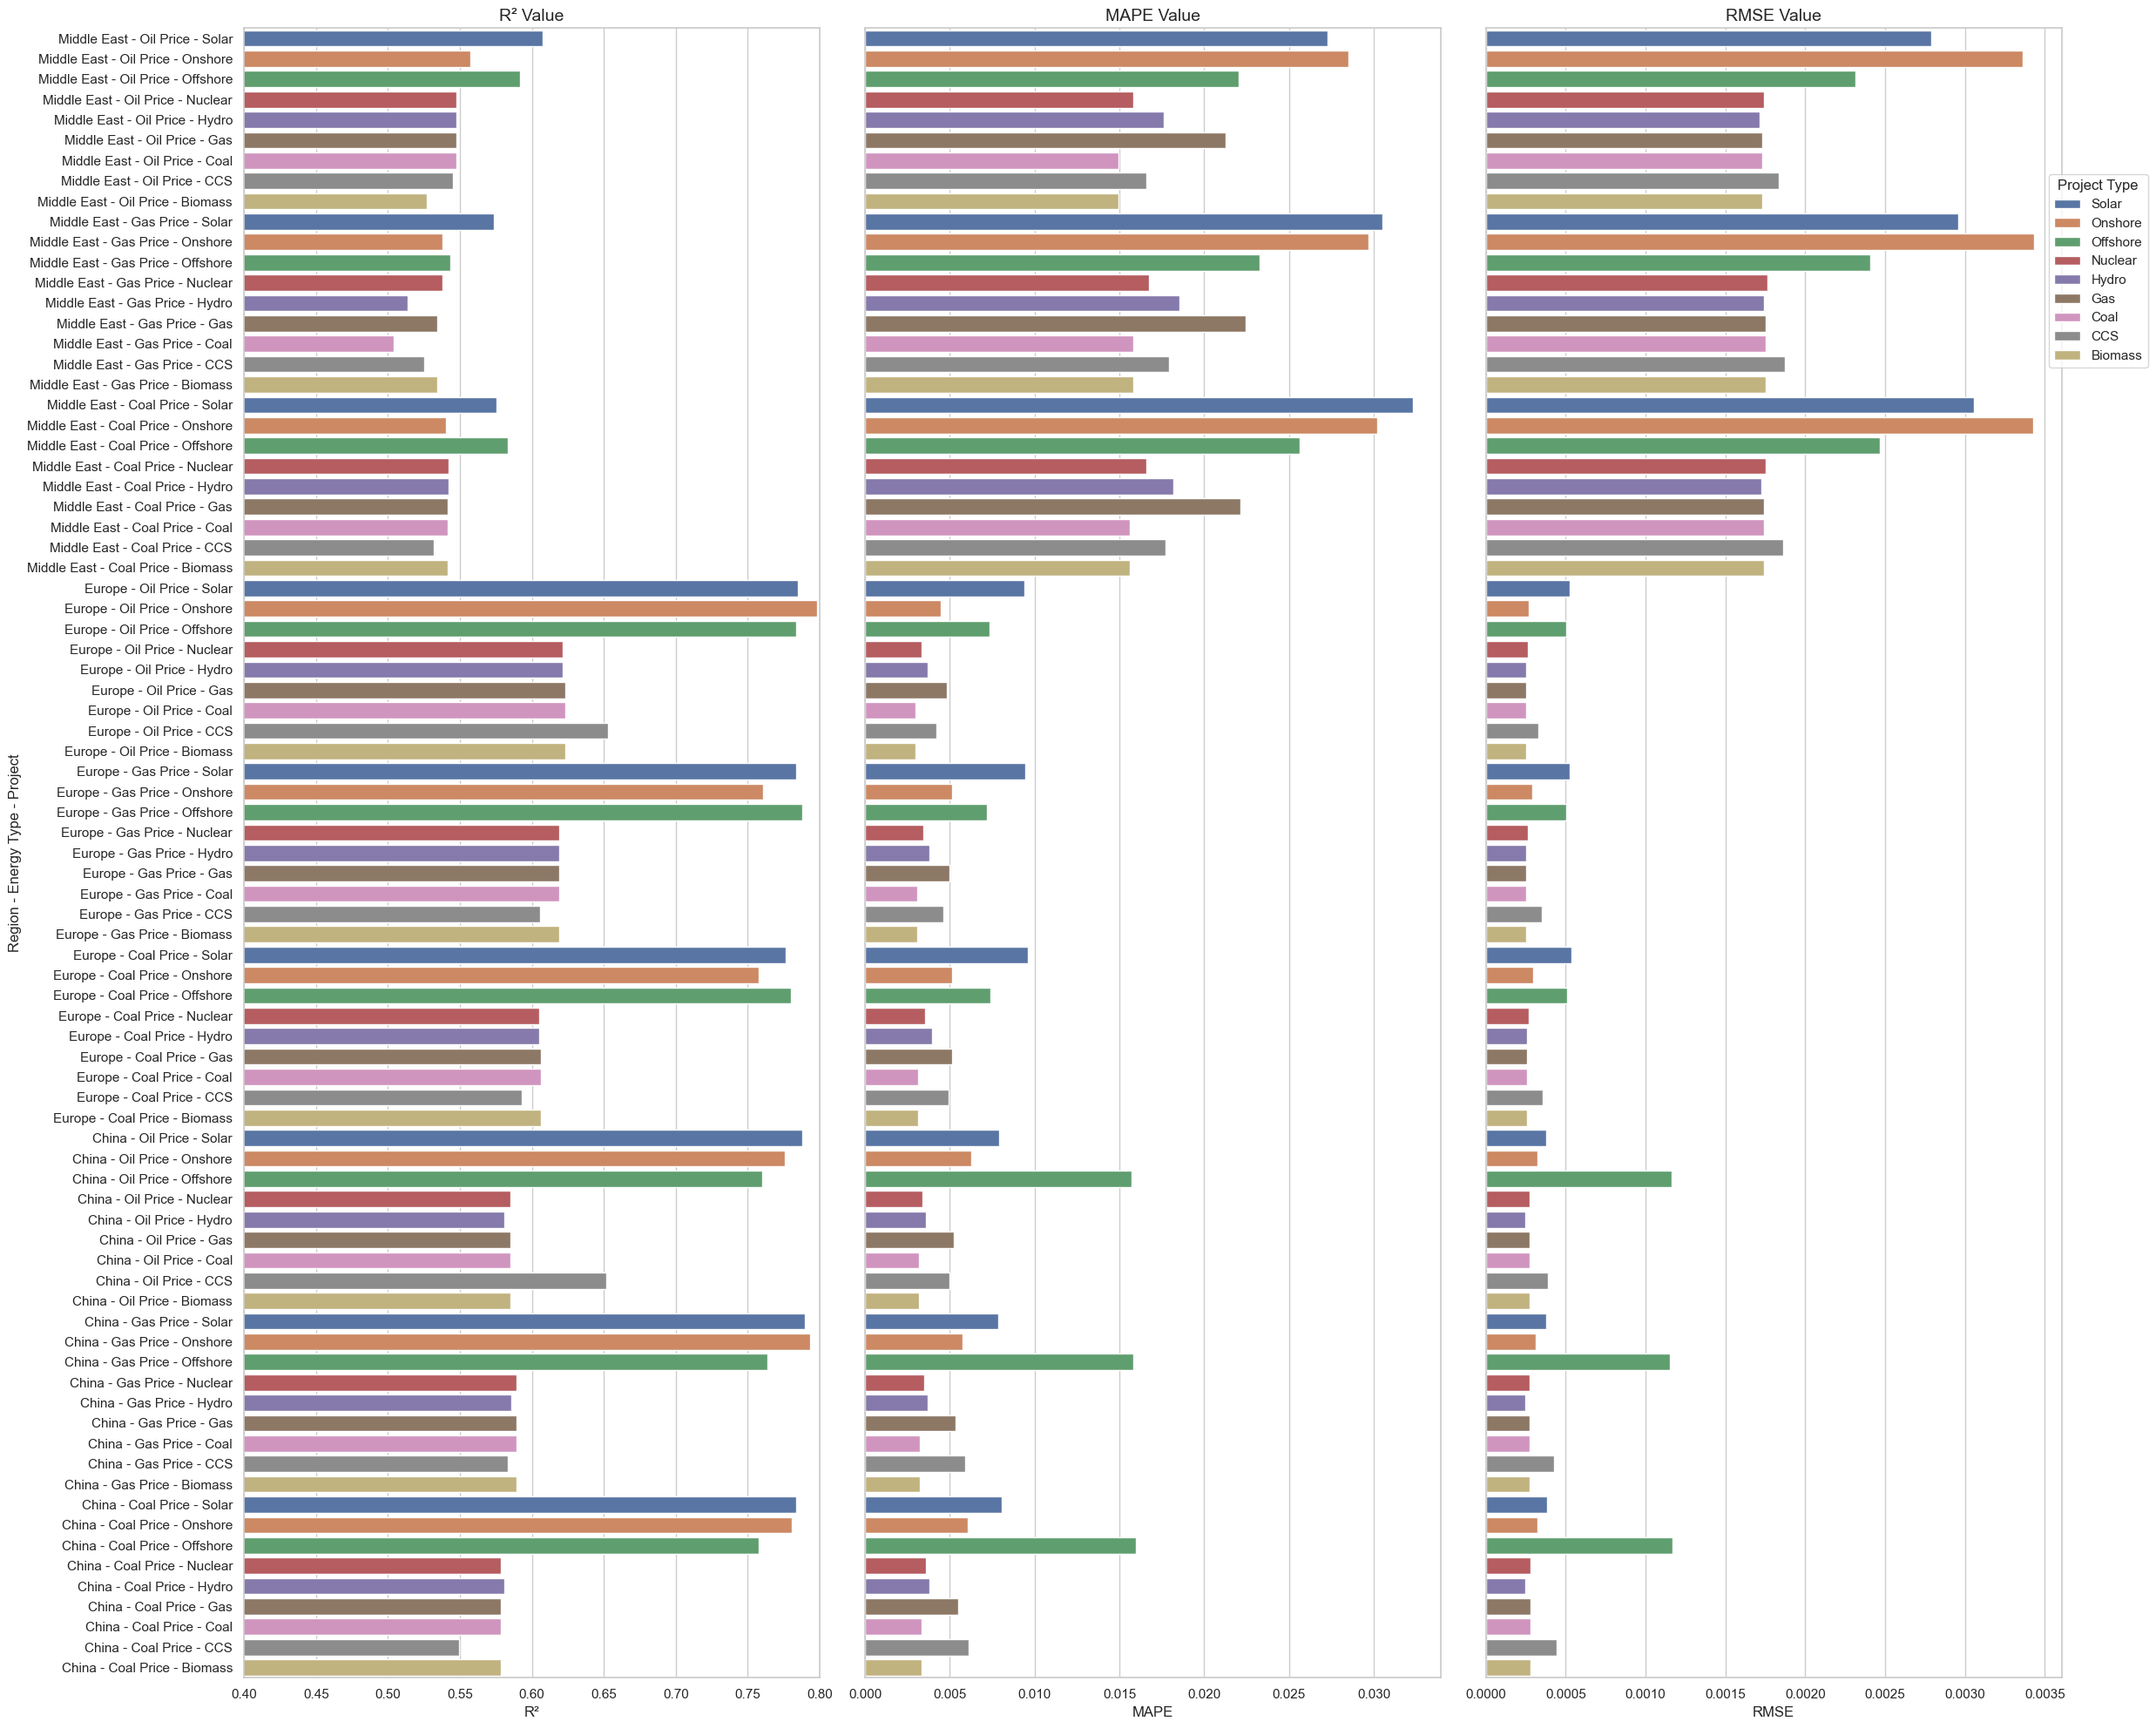
\includegraphics[width=0.98\textwidth]{figure.png}
    \caption{In-sample model performance for each project: comparison of $R^2$, MAPE, and RMSE for estimating WACC across various regions and energy transition projects.}
    \label{fig:result9}
\end{figure*}

\section{Results}

As shown in Fig.~\ref{fig:result9}, the experiment results demonstrate differences in WACC model fit across energy transition projects. Solar and wind (both onshore and offshore) projects demonstrate the highest model fit, with average $R^2$ values all exceeding 0.7. In contrast, other projects, including hydropower, biomass, and coal, exhibit lower model fit, with average $R^2$ values around 0.58.

From a regional perspective, model fit exhibits clear geographical characteristics. In major energy-importing regions like Europe and China, the model fit is higher, with average $R^2$ values of 0.67 and 0.65. Conversely, the model fit is lower in the Middle East, an energy-exporting region, where the average $R^2$ value is 0.55. This disparity is also reflected in the prediction error, as the Middle East's average MAPE (0.0209) is substantially higher than that of Europe (0.0050) and China (0.0061), indicating larger relative prediction errors.

\subsection{Robustness Checks}

The additional holdout and rolling-origin checks support a more cautious interpretation of these results. The main results in Fig.~\ref{fig:result9} summarize in-sample fit within the constructed 2026-2035 panel, while the time-split tests examine how stable the fitted relationships remain when later years are held out. The fixed holdout uses 2026-01 to 2032-12 as the training period and 2033-01 to 2035-12 as the test period. Rolling-origin validation trains through one calendar year and tests the following year.

Across these checks, MAPE remains small for level and trend specifications, but $R^2$ is often unstable because the test-period WACC variation is narrow. Therefore, the paper treats the estimated relationships as predictive sensitivity and stress-scenario evidence rather than as formal causal effects. Table~\ref{tab:robustness} summarizes how the robustness outputs are used in interpreting the findings.

\begin{table}[t]
\centering
\caption{Robustness Checks Used for Interpretation}
\label{tab:robustness}
\scriptsize
\begin{tabular}{P{0.27\linewidth}P{0.30\linewidth}P{0.34\linewidth}}
\toprule
\textbf{Check} & \textbf{Setup} & \textbf{Interpretation} \\
\midrule
Fixed holdout & Train 2026-2032; test 2033-2035 & Later-year prediction is sensitive to specification; use the main $R^2$ values as scenario-fit evidence. \\
Rolling origin & Train through one year; test the next year & Percentage errors are small in level/trend specifications, but $R^2$ varies under narrow WACC ranges. \\
Incremental $R^2$ & Add fuel price and inflation beyond time trend & Positive cases occur for 8/27 China models, 6/27 Europe models, and 6/27 Middle East models (Ridge specifications). \\
Elasticity checks & Log-linear 10\% price shock conversion & Coefficients are interpreted as price-shock sensitivity, not causal effects. \\
\bottomrule
\end{tabular}
\end{table}

\section{Discussion}
\label{sec:discussion}

\subsection{Regional Differences}

\subsubsection{Europe}
The original European specifications have the strongest average in-sample fit ($R^2=0.670$). Europe's reliance on imported energy provides a relevant context for examining international price exposure. Rom\'an-Collado and Casado Ru\'iz identify energy dependence, economic activity, and efficiency as drivers of EU-27 energy imports over 2000--2020 \cite{ROMANCOLLADO2024108009}. Li and Leung examine links between energy prices, economic growth, and renewable-energy consumption in Europe \cite{LI20211712}. These studies support the regional context, rather than a specific WACC response inferred from the fit statistic.

\subsubsection{Structural Dependence and Policy Limitations}
Carbon pricing and renewable-energy policy shape the investment environment. The EU ETS literature emphasizes the importance of policy design and innovation incentives \cite{EUETS}, while the Renewable Energy Directive provides a framework for renewable deployment \cite{RenewableEnergyDirective}. Policy credibility and predictability matter for both investment risk and expected returns \cite{POLZIN20191249}. These mechanisms motivate explicit policy scenarios in future financing analysis.

\subsubsection{External Shocks and Financial Risks}
The European energy crisis illustrates the importance of energy security and storage planning \cite{WEI2024110522}. Fiscal instruments can also alter the pass-through of energy-price shocks to inflation and output in energy-importing economies \cite{GLOCKER2024103201}. Financing instruments provide a complementary channel: green-bond certification and issuance can influence investor participation and the credibility of environmental commitments \cite{ehlers2017green,flammer2021corporate}. The present regressions do not quantify the separate effects of these policies or instruments.

\subsubsection{China}
China's original average fit is $R^2=0.650$. Research finds time-varying spillovers between international and Chinese energy and commodity markets \cite{SUN2022121642,WANG2023128724}. These links provide a rationale for including international fuel-price signals in regional financing analysis.

\subsubsection{Import Dependence}
Ben-Salha et al. find long-run relationships between fossil fuel prices and renewable-energy consumption in China, but no significant short-run effects in their specification \cite{ben2022assessing}. Their results support a distinction between short-run price exposure and longer-run substitution toward renewables; they do not provide project-level WACC elasticities.

\subsubsection{Government Intervention}
Price regulation can modify the domestic consequences of international energy-market changes. He and Lin model the economic and emissions effects of natural-gas price control in China \cite{HE2017524}. Policy design, public finance, and risk mitigation are therefore relevant considerations when interpreting regional financing conditions \cite{POLZIN20191249,duma2023risk}.

\subsubsection{Middle East}
The original Middle Eastern specifications have a lower average fit ($R^2=0.547$). Oil dependence, diversification, and domestic pricing institutions provide possible contextual explanations, but their separate roles are not identified by the regression. Karanfil and Omgba examine structural factors that shape export diversification in oil-dependent economies \cite{karanfil2023energy}.

\subsubsection{Economic Structure}
Fossil fuel revenues may support public investment and financing capacity, while also exposing public budgets to commodity cycles. A fiscal buffer is therefore a hypothesis to examine using sovereign-finance and project-level data. The corrected sensitivity diagnostics show why this distinction matters: lower model fit in the Middle East can coexist with larger estimated price-response coefficients in some technologies (Appendix Table~\ref{tab:appendix-elasticities}).

\subsubsection{Institutional Design}
Fattouh and El-Katiri document the importance and economic trade-offs of energy subsidies in the Middle East and North Africa \cite{FATTOUH2013108}. Such arrangements can affect domestic price exposure and investment incentives. Their effects on renewable-project financing should be evaluated together with contract design, counterparty risk, and guarantees \cite{duma2023risk}, rather than inferred solely from regional fit differences.

\subsection{Transmission Diagnostics}
Historical Granger-style tests use first-differenced macroeconomic targets and log-differenced annual fuel prices. Table~\ref{tab:granger} reports selected lagged associations: coal-price changes with China's real interest rate at one- and two-year lags, gas-price changes with China's real interest rate at one-year lag, and gas-price changes with European inflation at two-year lag. The reported $p$-values are unadjusted exploratory diagnostics; the complete tested set is provided in the repository. The China inflation--coal result ($p=0.09394$) is not significant at the 5\% level. These tests examine the plausibility of macroeconomic transmission channels and do not identify project-level WACC effects.

\begin{table}[t]
\centering
\caption{Selected Historical Transmission Diagnostics}
\label{tab:granger}
\footnotesize
\begin{tabular}{llrr}
\toprule
\textbf{Region/target} & \textbf{Fuel} & \textbf{Lag} & \textbf{$p$-value} \\
\midrule
China real interest rate & Coal & 1 & 0.00018 \\
China real interest rate & Coal & 2 & 0.00691 \\
China real interest rate & Gas & 1 & 0.01915 \\
Europe inflation & Gas & 2 & 0.00952 \\
China inflation & Coal & 1 & 0.09394 \\
\bottomrule
\end{tabular}
\end{table}

\subsection{Environmental Implications of Financial Sensitivity}
Financing conditions can influence the affordability and timing of renewable investment. Prior modeling shows that regional differences in capital costs can materially change decarbonization pathways \cite{ameli2021higher,calcaterra2024reducing}. The present study adds a framework for comparing fuel-price and inflation signals across regional WACC scenarios. Translating its outputs into deployment, emissions, or household-price effects requires a linked investment or energy-system model.

\subsection{Regional Community Impact}
Reliable energy finance is relevant to affordability and a just transition. European research documents substantial geographical differences in energy poverty \cite{bouzarovski2017energy}, and the OECD emphasizes aligning local climate finance with inclusive development \cite{oecd2021financing}. These concerns motivate analysis of financing conditions in Europe, China, and the Middle East. Household welfare, employment, and energy access are potential applications of the framework rather than outcomes measured here.

\subsection{Climate Finance \& Policy}
For Europe, policy credibility, predictable revenue arrangements, and risk-transfer instruments are relevant options for stabilizing renewable investment conditions \cite{POLZIN20191249,duma2023risk}. For China, the interaction between international price signals, domestic price regulation, and public financing merits explicit comparison across policy scenarios \cite{HE2017524}. For oil-dependent economies, diversification and the design of domestic energy-pricing arrangements remain central considerations \cite{karanfil2023energy,FATTOUH2013108}. Across regions, the framework is most useful as a structured comparison of assumptions and financing exposures, alongside institutional and project-level evidence.

\section{Conclusion and Future Work}

This study introduces a three-stage machine learning model to assess the effects of fossil fuel price volatility on the WACC of energy transition projects. The findings emphasize that achieving the 1.5$^\circ$C target requires region-specific climate finance solutions. Policymakers and investors need to tailor their strategies to address the unique challenges posed by fossil fuel price volatility, since this can promote renewable energy investments that remain financially viable and resilient amid global market shifts. The results also reinforce the SDG framing introduced at the outset: de-risking clean-energy finance supports affordable and clean energy (SDG 7), climate action (SDG 13), open and reproducible innovation infrastructure (SDG 9), and cross-regional research partnerships (SDG 17).

While this study provides some insights into the financial dynamics of the energy transition, further research is also needed. Initially, some datasets and assumptions rely on secondary sources. Future work could enhance the robustness of these findings by incorporating firm-level financial data and longer regional panels. Additionally, future work could transition from quantifying predictive sensitivity to formal causal inference, using techniques such as fixed effects, instrumental variables, or Structural Equation Models to handle policy variables, financial mechanisms, and technological learning rates. Finally, the framework itself can be enhanced by benchmarking against advanced architectures such as Transformers or state-space models and propagating uncertainty across all three stages, including the GPR predictive variance, for uncertainty quantification and stress-testing.

\section*{Acknowledgment}
OpenAI Codex assisted language and consistency revisions throughout the manuscript, preparation of Fig.~\ref{fig:tensor-framework}, and correction of the sensitivity-analysis code. Funding and presenting-author acknowledgments are stated on the first page.


\bibliographystyle{IEEEtran}
\bibliography{references}

\clearpage
\appendices
\section{Reproducibility and Data Supplement}

This appendix expands the reproducibility checklist into a data and configuration supplement. It records the files used in each stage, the cleaned WACC panel coverage, the main model settings, and the additional diagnostic outputs used to interpret the results. The purpose is to make the IEEE version self-contained while preserving the original three-stage workflow.

\subsection{Repository and Execution Environment}

\begingroup\raggedright
All experiments follow the repository workflow used in the original submission. The primary notebooks are \texttt{Price\_Prediction.ipynb}, \texttt{Prediction\_Inflation.ipynb}, and \texttt{Impact\_FossilFuel.ipynb}. The revision diagnostics are generated by \texttt{code/revision\_experiments.py}. The versioned source and corrected diagnostics are available in the \href{https://github.com/GreenComp-ERC/ImpactOfFossilFeulPrice}{organization repository}. Experiments were run on macOS with an Apple arm64 10-core CPU and 16GB RAM. The original notebooks specify Python, AutoGluon, TensorFlow/Keras, and scikit-learn. The corrected diagnostic script depends on pandas, NumPy, and openpyxl; its rerun environment and checks are recorded in the versioned repository.\par\endgroup

\begin{table}[!ht]
\centering
\caption{Files Included in the IEEE Source Folder}
\label{tab:appendix-file-inventory}
\scriptsize
\begin{tabular}{P{0.24\columnwidth}P{0.28\columnwidth}P{0.36\columnwidth}}
\toprule
\textbf{Folder} & \textbf{File} & \textbf{Purpose} \\
\midrule
\texttt{figures/} & \texttt{LSTM.png} & Stage 1 architecture figure \\
\texttt{figures/} & \texttt{Accuracy.png} & Oil price forecast comparison \\
\texttt{figures/} & \texttt{figure.png} & Stage 3 regional/project metrics \\
\texttt{figures/} & Tensor framework PDF & First-page tensor workflow figure \\
\texttt{figures/} & Methodology relations PDF & Three-stage method and model-relation figure \\
\texttt{data/} & Stage 1 metrics & Forecast metric table \\
\texttt{data/} & Stage 3 holdout & 2033-2035 holdout checks \\
\texttt{data/} & Rolling metrics & Rolling-origin checks \\
\texttt{data/} & Shock elasticities & 10\% price-shock sensitivity \\
\texttt{data/} & Granger diagnostics & Transmission diagnostics \\
\bottomrule
\end{tabular}
\end{table}

\subsection{Data Sources and Cleaning}

Stage 1 uses historical coal, gas, and oil prices from World Bank commodity data. Stage 2 uses macroeconomic indicators, including consumer price inflation, gross domestic product growth, unemployment, real interest rate, money supply, and trade-balance indicators. Stage 3 combines predicted fuel prices and inflation with WACC projections derived from Calcaterra et al. The cleaned WACC inputs keep a common monthly horizon from 2026-01 to 2035-12 for China, Europe, and the Middle East.

\begin{table}[!ht]
\centering
\caption{Cleaned WACC Panel Coverage}
\label{tab:appendix-cleaned-wacc}
\scriptsize
\begin{tabular}{lrrrr}
\toprule
\textbf{Region} & \textbf{Raw} & \textbf{Clean} & \textbf{Horizon} & \textbf{Mean Fix} \\
\midrule
China & 120 & 120 & 2026-2035 & 0.000 \\
Europe & 120 & 120 & 2026-2035 & 1.090 \\
Middle East & 180 & 120 & 2026-2035 & 1.031 \\
\bottomrule
\end{tabular}
\vspace{2pt}

\raggedright\scriptsize
\textit{Note:} ``Mean Fix'' is the mean absolute correction to the inflation column, in percentage points. Missing values after cleaning are zero for all regions. The original Europe and Middle East workbooks used China's inflation series; cleaning replaces it with the respective regional forecasts. The original AutoGluon fit summaries remain archived separately from the cleaned-panel diagnostics.
\end{table}

\begin{table}[!ht]
\centering
\caption{Core Variables Used by Stage}
\label{tab:appendix-core-variables}
\scriptsize
\begin{tabular}{P{0.23\columnwidth}P{0.35\columnwidth}P{0.30\columnwidth}}
\toprule
\textbf{Stage} & \textbf{Variables} & \textbf{Role} \\
\midrule
Stage 1 & Fuel price, month sine/cosine, rolling averages & Price forecasting input and target \\
Stage 2 & CPI inflation, GDP growth, unemployment, real interest rate, money supply, trade indicators & Inflation forecasting input and target \\
Stage 3 & Coal, gas, oil price; inflation; WACC by project type & WACC sensitivity estimation \\
Diagnostics & Log price differences; differenced inflation and interest rates & Transmission mechanism checks \\
\bottomrule
\end{tabular}
\end{table}

\subsection{Model Configuration}

The Stage 1 LSTM-GPR model first learns temporal fuel-price patterns and then smooths the neural forecasts with Gaussian Process Regression. The GPR uses a constant kernel multiplied by a radial basis function kernel plus a white-noise term, with \texttt{alpha=0.01}, \texttt{n\_restarts\_optimizer=10}, and \texttt{random\_state=42}. Stage 2 uses an LSTM and feed-forward inflation predictor with an ensemble size of five. Stage 3 uses AutoGluon-Tabular with bagging and stacking enabled.

\begin{table}[!ht]
\centering
\caption{Stage 1 Price-Forecasting Settings}
\label{tab:hyperparameter-summary}
\label{tab:appendix-stage1-settings}
\scriptsize
\begin{tabular}{P{0.48\columnwidth}P{0.36\columnwidth}}
\toprule
\textbf{Parameter} & \textbf{Value} \\
\midrule
Time step & 12 months \\
Input scaling & Min-max, range (0, 1) \\
Conv1D filters / kernel & 80 / 3 \\
Bidirectional LSTM units & 128 \\
GRU units & 64 \\
Dense units & 80 \\
Dropout rates & 0.3, 0.5, 0.5 \\
Learning rate & 0.0005 \\
Epochs / batch size & 200 / 32 \\
Early stopping patience & 20 \\
GPR kernel & Constant $\times$ RBF + white noise \\
GPR optimizer restarts & 10 \\
GPR alpha / seed & 0.01 / 42 \\
\bottomrule
\end{tabular}
\end{table}

\begin{table}[!ht]
\centering
\caption{Stage 2 and Stage 3 Settings}
\label{tab:appendix-stage23-settings}
\scriptsize
\begin{tabular}{P{0.16\columnwidth}P{0.43\columnwidth}P{0.25\columnwidth}}
\toprule
\textbf{Stage} & \textbf{Parameter} & \textbf{Value} \\
\midrule
Stage 2 & Imputer neighbors & 3 \\
Stage 2 & Scaler & StandardScaler \\
Stage 2 & Lookback / time step & 4 \\
Stage 2 & Ensemble size & 5 \\
Stage 2 & LSTM units & 32 and 16 \\
Stage 2 & Dense units & 64 and 32 \\
Stage 2 & Regularization & L2(0.01) \\
Stage 2 & Epochs / batch size & 300 / 8 \\
Stage 2 & Validation split & 0.2 \\
Stage 3 & AutoGluon time limit & 600 seconds \\
Stage 3 & Bagging folds & 10 \\
Stage 3 & Stacking & auto stack \\
Stage 3 & GBM depth / learning rate & 3 / 0.01 \\
Stage 3 & CAT depth / learning rate & 3 / 0.01 \\
\bottomrule
\end{tabular}
\end{table}

\subsection{Forecasting and Robustness Outputs}

The archived oil-price comparison covers 47 observations in 2021--2024. Separate fixed-origin baseline forecasts use training data through 2020. The LSTM-GPR series has the smallest errors among the four archived comparison outputs. In Stage 3, the holdout split trains on 2026-01 to 2032-12 and tests on 2033-01 to 2035-12. Rolling-origin checks train through one calendar year and test the following year. These checks are used to separate predictive sensitivity from causal identification.

\begin{table}[!ht]
\centering
\caption{Stage 1 Oil-Price Forecast Metrics}
\label{tab:appendix-stage1-metrics}
\scriptsize
\begin{tabular}{lrrrr}
\toprule
\textbf{Model} & \textbf{$R^2$} & \textbf{MAPE} & \textbf{RMSE} & \textbf{MAE} \\
\midrule
LSTM-GPR & 0.963 & 0.0186 & 2.416 & 1.425 \\
LightGBM & 0.932 & 0.0299 & 3.267 & 2.464 \\
XGBoost & 0.729 & 0.0644 & 6.546 & 5.273 \\
SARIMA & -10.206 & 0.4839 & 42.069 & 39.449 \\
\bottomrule
\end{tabular}
\end{table}

\begin{table}[!ht]
\centering
\caption{Stage 3 Validation Summary}
\label{tab:appendix-validation}
\scriptsize
\begin{tabular}{lrrr}
\toprule
\textbf{Region} & \textbf{Holdout MAPE} & \textbf{Rolling MAPE} & \textbf{Positive Inc.} \\
\midrule
China & 0.0130 & 0.0100 & 8/27 \\
Europe & 0.0102 & 0.0078 & 6/27 \\
Middle East & 0.0555 & 0.0436 & 6/27 \\
\bottomrule
\end{tabular}
\vspace{2pt}

\raggedright\scriptsize
\textit{Note:} Holdout values use the Ridge inflation-trend or time-only specification with the lowest mean MAPE by region. Rolling values report the lowest mean MAPE across stable level/trend specifications. ``Positive Inc.'' counts models where adding fuel price and inflation improves out-of-sample $R^2$ over a time trend.
\end{table}

\subsection{Scenario Sensitivity and Transmission Diagnostics}

The price-shock table converts log-linear elasticities into average basis-point changes in WACC under a 10\% fuel-price shock. These values are conditional scenario sensitivities around the modeled WACC mean. The coefficient on log price is divided by the standard deviation of log price before conversion to original units. After reversing input standardization, the largest absolute responses in the cleaned panel occur in Middle East coal-price specifications. The table reports exact log-linear 10\% shock conversions around the modeled mean.

\begin{table}[!ht]
\centering
\caption{Largest 10\% Price-Shock Sensitivities}
\label{tab:appendix-elasticities}
\scriptsize
\begin{tabular}{llrr}
\toprule
\textbf{Region/Project} & \textbf{Fuel} & \textbf{WACC} & \textbf{bp} \\
\midrule
Middle East Onshore & Coal & 8.56\% & -26.058 \\
Middle East Solar & Coal & 7.54\% & -23.359 \\
Middle East Offshore & Coal & 7.60\% & -20.513 \\
Middle East Nuclear & Coal & 7.31\% & -14.954 \\
Middle East CCS & Coal & 7.54\% & -14.843 \\
Middle East Biomass & Coal & 7.66\% & -14.815 \\
Middle East Hydro & Coal & 6.52\% & -14.638 \\
China Offshore & Coal & 5.76\% & -7.500 \\
\bottomrule
\end{tabular}
\end{table}

\begin{table}[!ht]
\centering
\caption{Selected Granger-Style Transmission Diagnostics}
\label{tab:appendix-granger}
\scriptsize
\begin{tabular}{P{0.35\columnwidth}lrr}
\toprule
\textbf{Target} & \textbf{Fuel} & \textbf{Lag} & \textbf{$p$} \\
\midrule
China real interest rate & Coal & 1 & 0.00018 \\
China real interest rate & Coal & 2 & 0.00691 \\
Europe inflation & Gas & 2 & 0.00952 \\
China real interest rate & Gas & 1 & 0.01915 \\
China inflation & Coal & 1 & 0.09394 \\
\bottomrule
\end{tabular}
\vspace{2pt}

\raggedright\scriptsize
\textit{Note:} Diagnostics use first-differenced macro targets and log-differenced annual fuel prices. They indicate plausible transmission channels rather than structural causal identification.
\end{table}

\subsection{Replication Sequence}

To reproduce the manuscript results, first run the fuel-price preprocessing and prediction notebooks to generate price forecasts. Second, run the inflation prediction notebook to obtain macroeconomic covariates for the 2026-2035 horizon. Third, merge price, inflation, and WACC panels by region and project type and run the AutoGluon WACC evaluation. Finally, run the revision script to regenerate the holdout metrics, rolling-origin metrics, price-shock elasticities, and transmission diagnostics copied into the IEEE source tree. The raw WACC files are preserved, while cleaned regional inputs are written separately so the revision process remains auditable.


\end{document}
